\chapter{Terrain Classification for Hexapod Robot AMOS II} \label{chap:terrain_classification}

The classification problem in this thesis relates to AMOS II, an open-source multi sensori-motor robotic platform (see \cref{img:amosii}). The task is to classify various terrain types based on proprioceptive (joint angles) and tactile (ground contact) sensors. The overall process is based on simulation data and as stated in \cref{chap:kitt_nn}, feedforward neural networks are used for classification.

\section{Overall Process Summary} \label{sec:overall_process_summary}
The overall process consists of several modules. The workflow is illustrated in \cref{img:terrain_overall_simple} (a more detailed diagram can be found in \cref{img:app:terrain_classification_process}).

\begin{figure}[H]
  \centering
  \includegraphics[width=0.5\textwidth]{terrains_overall_simple.png}
  \caption{Terrain Classification: overall process diagram}
  \label{img:terrain_overall_simple}
\end{figure}

The very first step is to make the AMOS II simulation run (\cref{ssec:app:lpzrobots_sim}). Then a simple tripod gait controller is implemented (\cref{ssec:tripod_gait_controller}). To generate various terrain types, the number of variable terrain features and their ranges are determined (\cref{ssec:terrain_features}). Based on these features (parameters), a number of virtual terrains is defined (\cref{ssec:features_determination}) and an optimality of these parameters is briefly analysed (\cref{ssec:terrains_analysis}).

Next, AMOS II (its simulation alternative) is forced to walk on every defined terrain type several times and for a sufficiently long period of time and the data from all proprioceptors are saved. This data is then verified and failing experiments are removed. The data acquisition step is parameterized by a standard deviation of an additive (Guassian) terrain noise and is run for several values.

Having the clean simulation data from all sensors, a feature vector structure is determined. Then a Gaussian signal noise is added. 

Finally, a dataset is created by splitting all the data into training, validation and testing sets. As it is indicated in \cref{img:app:terrain_classification_process}, several datesets and several classifiers are generated during the process. 

The dataset packages may differ in these parameters:
\begin{itemize}
\item terrain types included (number of classes)
\item sensors on input
\item samples length (number of simulation timesteps)
\item terrain noise and signal noise
\item number of samples
\end{itemize}

The trained networks may differ in the following parameters:
\begin{itemize}
\item dataset that the network has been tested on
\item neural network structure
\item learning parameters: learning rate and number of epochs
\end{itemize}

Finally, an optimal neural network classifier is found. The optimal network is then pruned by the algorithm developed in \cref{sec:network_pruning_algorithm}. The classification performance of developed tools is compared to \textit{Scikitlearn-neuralnetwork} classification library \citep{misc:sknn}.

\section{Experimental Environment Specification}
The final objective of this thesis was to implement an online terrain classifier for selection of optimal walking gait on real hexapod robot AMOS II. Therefore the real hexapod robot is presented in the following section \ref{ssec:amosii}.

However, as already stated above, the proposed approach will be evaluated using simulated robot in a virtual environment. In this case, \textit{LPZ Robots simulator} \citep{misc:lpzrobots} was used and a description is given in section 6.2.2.

\subsection{Hexapod Robot AMOS II} \label{ssec:amosii}
The \textit{AMOS II} abbreviation stands for Advanced Mobility Sensor Driven-Walking Device - version II \citep{misc:amosii}. It is a biologically inspired hardware platform of size 30x40x20 cm and weight 5.8 Kg (see \cref{img:amosii}). It is mainly used to study a neural control, memory and learning for machines with many degrees of freedom. The body and parts of the robot are inspired by a cockroach.

\begin{figure}[H]
  \centering
  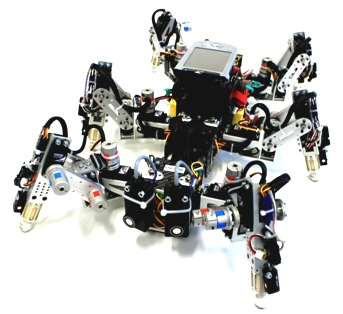
\includegraphics[width=343px]{amosii}
  \caption{AMOS II. \citep{misc:amosii}}
  \label{img:amosii}
\end{figure}

A wide range of sensors (for instance infra-red, reflexive optical, light-dependent, laser, camera, inclinometer sensors) allows AMOS II to perform several kinds of autonomous behaviour including foothold searching, elevator reflex (swinging a leg over obstacles), self-protective reflex (standing in an upside-down position), obstacle avoidance, escape responses etc. \citep{misc:amosii}. However, only proprioceptive and tactile sensors are important for this study. Therefore, we focus on joint angle sensors and foot contact sensors. All of them are located on robot's legs. The leg structure is shown in \cref{img:amosii_leg}.

\begin{figure}[H]
  \centering
  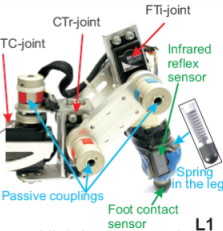
\includegraphics[width=0.5\textwidth]{amosii_leg}
  \caption{Structure of the AMOS's leg. \citep{misc:amosii}}
  \label{img:amosii_leg}
\end{figure}

As shown in \cref{img:amosii} and \cref{img:amosii_leg}, the robot has \textit{6 foot contact sensors} in total, one on each leg. Each of them returns a value from range $ [0.0, 1.0] $ depending on how strong the foot contact is, i.e., it is equal $ 1.0 $ if the robot stands on the leg with its full weight and it equals $ 0.0 $ when the leg is in the air.

There are three joints on each of the robot's legs. The thoraco-coxal (TC-) joint is responsible for forward/backward movements. The coxa-trochanteral (CTr-) joint enables elevation and depression of the leg and the last one, femur-tibia (FTi-) joint is used for extension and flexion of the tibia.

These joints are physically actuated by standard servo motors. Angles of the joints are measured by the servo motors and are considered as propriceptive sensors. As AMOS II has six legs and there are three joints on each leg, there are \textit{18 angle sensors} in total. There is also one backbone joint angle, however, as this one is not implemented in the simulation (see \cref{ssec:app:lpzrobots_sim}), it is omitted in this work.

In \cref{tab:proprioceptors} all the propriceptive sensors, their abbreviations and original ranges are listed. The ranges are based on the individual servo motors locations and are manually set to avoid collisions. In \cref{sec:feature_vector_compilation} a normalization of these ranges is discussed.

Robot actuators (servo motors) can generate movements of variable compliance by utilizing a virtual muscle model (see \cite{misc:amosii} for details). 

\begin{table}[H]
\centering
\caption{Summary of proprioceptive sensors of AMOS II hexapod robot}
\label{tab:proprioceptors}
\begin{tabular}{|l|l|c|}
\hline
\textit{abbr.} & \multicolumn{1}{c|}{\textit{sensor description}} & \textit{original range} \\ \hline
\textbf{ATRf}         & Angle sensor, Thoraco joint, Right front leg     & {[}-0.5, 0.5{]}         \\ \hline
\textbf{ATRm}         & Angle sensor, Thoraco joint, Right middle leg    & {[}-0.5, 0.5{]}         \\ \hline
\textbf{ATRh}         & Angle sensor, Thoraco joint, Right hind leg      & {[}-0.5, 0.5{]}         \\ \hline
\textbf{ATLf}         & Angle sensor, Thoraco joint, Left front leg      & {[}-0.5, 0.5{]}         \\ \hline
\textbf{ATLm}         & Angle sensor, Thoraco joint, Left middle leg     & {[}-0.5, 0.5{]}         \\ \hline
\textbf{ATLh}         & Angle sensor, Thoraco joint, Left hind leg       & {[}-0.5, 0.5{]}         \\ \hline
\textbf{ACRf}         & Angle sensor, Coxa joint, Right front leg        & {[}-0.5, 0.5{]}         \\ \hline
\textbf{ACRm}         & Angle sensor, Coxa joint, Right middle leg       & {[}-0.5, 0.5{]}         \\ \hline
\textbf{ACRh}         & Angle sensor, Coxa joint, Right hind leg         & {[}-0.5, 0.5{]}         \\ \hline
\textbf{ACLf}         & Angle sensor, Coxa joint, Left front leg         & {[}-0.5, 0.5{]}         \\ \hline
\textbf{ACLm}         & Angle sensor, Coxa joint, Left middle leg        & {[}-0.5, 0.5{]}         \\ \hline
\textbf{ACLh}         & Angle sensor, Coxa joint, Left hind leg          & {[}-0.5, 0.5{]}         \\ \hline
\textbf{AFRf}         & Angle sensor, Femur joint, Right front leg       & {[}-0.5, 0.5{]}         \\ \hline
\textbf{AFRm}         & Angle sensor, Femur joint, Right middle leg      & {[}-0.5, 0.5{]}         \\ \hline
\textbf{AFRh}         & Angle sensor, Femur joint, Right hind leg        & {[}-0.5, 0.5{]}         \\ \hline
\textbf{AFLf}         & Angle sensor, Femur joint, Left front leg        & {[}-0.5, 0.5{]}         \\ \hline
\textbf{AFLm}         & Angle sensor, Femur joint, Left middle leg       & {[}-0.5, 0.5{]}         \\ \hline
\textbf{AFLh}         & Angle sensor, Femur joint, Left hind leg         & {[}-0.5, 0.5{]}         \\ \hline
\textbf{FRf}          & Foot contact sensor, Right front leg             & {[}0.0, 1.0{]}          \\ \hline
\textbf{FRm}          & Foot contact sensor, Right middle leg            & {[}0.0, 1.0{]}          \\ \hline
\textbf{FRh}          & Foot contact sensor, Right hind leg              & {[}0.0, 1.0{]}          \\ \hline
\textbf{FLf}          & Foot contact sensor, Left front leg              & {[}0.0, 1.0{]}          \\ \hline
\textbf{FLm}          & Foot contact sensor, Left middle leg             & {[}0.0, 1.0{]}          \\ \hline
\textbf{FLh}          & Foot contact sensor, Left hind leg               & {[}0.0, 1.0{]}          \\ \hline
\end{tabular}
\end{table}

It is possible to generate various gaits using joint actuators and robot's neural locomotion control. The gait controller used to generate robot locomotion is described in \cref{ssec:tripod_gait_controller}.

\subsection{AMOS II Simulation} \label{ssec:amosii_sim}
The \textit{lpzrobots} project, developed by a research group at the University of Leipzig \citep{misc:lpzrobots} under GPL license, is used for AMOS II virtual representation. Some implementation details are discussed in \cref{ssec:app:lpzrobots_sim}. The project modules important for this study are shown in \cref{img:lpzrobots_repos}.

With reference to \cref{app:code_documentation}, the \textit{main.cpp} file from \path{root/simulation/mbulinai22015-gorobots_edu-fork/practices/amosii} directory can be called as the main simulation file for purposes of the thesis. It sets up the environment with initial parameters:

\begin{itemize}
\item $ controlinterval = 10 $
\item $ simstepsize = 0.01 $
\end{itemize}

This results in setting the simulation sensitivity to \textit{10 steps} per second.

\begin{figure}[H]
  \centering
  \includegraphics[width=1.0\textwidth]{lpzrobots_repos}
  \caption{Structure of the two repositories: LPZRobots and GoRobots. \citep{misc:lpzrobots}}
  \label{img:lpzrobots_repos}
\end{figure}

The initial robot position in the map is chosen randomly in order to generate a different route everytime the simulation is launched. The robot fixator, which is originally implemented for AMOS II, is removed, so the robot starts walking right after the simulation is launched.

The \textit{main.cpp} file contains all terrain types parameters introduced in \cref{ssec:features_determination}. The required terrain to be simulated is then passed to this file as an argument. Additionally, the standard deviation value of Gaussian terrain noise (details in \cref{ssec:terrain_noise}) is set as another argument. 

Finally, the file is ready to take one more argument, which is a simulation noise represented by a float number. In this study it is fixed to zero though and only the terrain noise combined with a signal noise is used.

The virtual vizualization of AMOS II is illustrated in \cref{img:amosii_sim}.

\begin{figure}[H]
  \centering
  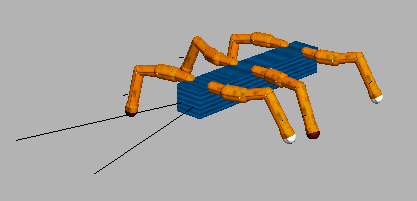
\includegraphics[width=0.8\textwidth]{amosii_sim}
  \caption{Virtual alternative for AMOS II.}
  \label{img:amosii_sim}
\end{figure}

Besides the backbone joint, all AMOS II actuators, proprioceptive and tactile sensors are modeled in the simulation and \textit{LpzRobots} framework is considered to provide an accurate simulated model of AMOS II.

\subsection{Tripod Gait Controller} \label{ssec:tripod_gait_controller}
The main motivation for the terrain classification is to adjust the current robot's gait accordingly and this way save some energy. In this work a \textit{tripod} gait (three legsg touching ground when walking) is used for classification. The tripod pattern is the fastest and most common gait for hexapods.

To generate the tripod gait, a central pattern generator (CPG) is used \citep{unpub:ai3_lec3}. It is implemented as a 2-neuron neural network as shown in \cref{img:two_neuron_network}.

\begin{figure}[H]
  \centering
  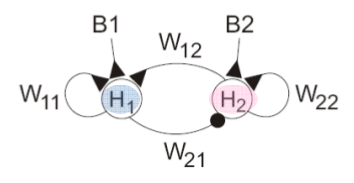
\includegraphics[width=0.5\textwidth]{two_neuron_network}
  \caption{2-neuron network oscillator \citep{unpub:ai3_lec3}}
  \label{img:two_neuron_network}
\end{figure}

The initial conditions and parameters of the implemented controller are shown in \cref{tab:tripod_controller_init}.

\begin{table}[H]
\centering
\caption{Initialization of \textit{tripod\_controller.h} (see \cref{app:code_documentation})}
\label{tab:tripod_controller_init}
\begin{tabular}{|l|c|l|}
\hline
\multicolumn{1}{|c|}{\textit{parameter}} & \textit{initial value} & \multicolumn{1}{c|}{\textit{description}} \\ \hline
$ aH_1 $                            & 0.0                    & activity of neuron $ H_1 $                     \\ \hline
$ aH_2 $                            & 0.0                    & activity of neuron $ H_2 $                     \\ \hline
$ oH_1 $                            & 0.001                  & output of neuron $ H_1 $                       \\ \hline
$ oH_2 $                            & 0.001                  & output of neuron $ H_2 $                       \\ \hline
$ bH_1 $                            & 0.0                    & bias for neuron $ H_1 $                        \\ \hline
$ bH_2 $                             & 0.0                    & bias for neuron $ H_2 $                        \\ \hline
$ wH_1H_1 $                          & 1.4                    & weight of the synapse from $ H_1 $ to $ H_1 $       \\ \hline
$ wH_1H_2 $                          & 0.4                    & weight of the synapse from $ H_2 $ to $ H_1 $       \\ \hline
$ wH_2H_1 $                          & -0.4                   & weight of the synapse from $ H_1 $ to $ H_2 $       \\ \hline
$ wH_2H_2 $                           & 1.4                    & weight of the synapse from $ H_2 $ to $ H_2 $       \\ \hline
$ p_1 $                              & 0.35                   & parameter for Thoraco joints              \\ \hline
$ p_2 $                              & 0.3                    & parameter for Coxa joints                 \\ \hline
\end{tabular}
\end{table}

Then, during the simulation, robot's joints are controlled in every simulation step by performing three actions:

\begin{enumerate}
\item \textbf{The activation function application}
\begin{equation}
a_i(t+1) = \displaystyle\sum_{j=1}^{n} w_{ij}o_j(t) + b_i, i = 1, ..., n
\end{equation}

\item \textbf{The transfer function application}
\begin{equation}
f(a_i) = tanh(a_i) = \frac{2}{1+e^{-2a_i}} - 1
\end{equation}

\item \textbf{Joint settings}

With the reference to previous equations and variables names, the actuators are set as shown in \cref{img:tripod_illustration}. The \textit{femur} joints (red ones) stay unchanged (set to zero). This setting generates a tripod gait for AMOS II.

\begin{figure}[H]
  \centering
  \includegraphics[width=200px]{tripod_illustration}
  \caption{Schematic diagram of tripod gait controller}
  \label{img:tripod_illustration}
\end{figure}
\end{enumerate}

\section{Generation of Virtual Terrains} \label{sec:generation_of_virtual_terrains}
Since the verification is based on the simulation only, the goal is to design a virtual environment. For this purpose various terrain types need to be virtually simulated.

A terrain is defined by four parameters: \textit{roughness}, \textit{slipperiness}, \textit{hardness} and \textit{elasticity}. These parameters form a substance together (this process is described in \cref{ssec:app:terrain_construction_in_main.cpp}).

Besides these four parameters represented as a substance handle, a terrain constructor takes six more arguments (used in \cref{code:terrain_ground}):

\begin{description}
\item[terrain\_color] : simulation ground color
\item["rough1.ppm"] : an image in the .ppm format, a lowest common denominator color image file format \citep{misc:ppm}, a bitmap height file
\item[""] : texture image (not used)
\item[20] : walking area x-size 
\item[25] : walking area y-size
\item[terrain\_height] : maximum terrain height
\end{description}

\subsection{Terrain Features} \label{ssec:terrain_features}
Out of the listed ground parameters, some of them are picked up and being called \textit{terrain features}, as they define a specific terrain type.

Therefore, a virtual terrain type is defined by five features. Each of them is a float number from an empirically stated range \footnote{The upper range limits have been set up based on significant changes in the robot behaviour for various parameter values.}. (\cref{tab:terrain_features}).

\begin{table}[H]
\centering
\caption{Terrain features and their ranges}
\label{tab:terrain_features}
\begin{tabular}{|l|c|c|c|c|} \hline
             & min value & min meaning & max value & max meaning \\\hline
roughness    & 0.0       & smooth		& 10.0		& rough     \\\hline
slipperiness & 0.0       & friction		& 100.0		& slippy    \\\hline
hardness     & 0.0       & soft			& 100.0		& hard	    \\\hline
elasticity   & 0.0       & rigid		& 2.0		& elastic   \\\hline
height       & 0.0       & low			& 0.1		& high		 \\\hline
\end{tabular}
\end{table}

\subsection{Features Determination for Various Terrains} \label{ssec:features_determination}
To determine a terrain type, one has to come up with the five parameters from \cref{tab:terrain_features}.

In this work we use 14 terrain types. Their parameters (shown in \cref{tab:terrains_parameters}) have been set up manually. With respect to the feature ranges from \cref{tab:terrain_features}, the values have been normalized between 0 and 1.

\begin{table}[H]
\centering
\caption{Parameters of virtual terrain types}
\label{tab:terrains_parameters}
\begin{tabular}{|l|l|c|c|c|c|c|}
\hline
\textit{\#}                                       & \textit{terrain title} & \multicolumn{1}{l|}{\textit{roughness}} & \multicolumn{1}{l|}{\textit{slipperiness}} & \multicolumn{1}{l|}{\textit{hardness}} & \multicolumn{1}{l|}{\textit{elasticity}} & \multicolumn{1}{l|}{\textit{height}} \\ \hline
1                         & \textbf{carpet}        & 0.3                                     & 0.0                                        & 0.4                                    & 0.15                                     & 0.2                                  \\ \hline
2                         & \textbf{concrete}      & 1.0                                     & 0.0                                        & 1.0                                    & 0.0                                      & 0.0                                  \\ \hline
3                         & \textbf{foam}          & 0.5                                     & 0.0                                        & 0.0                                    & 1.0                                      & 0.7                                  \\ \hline
4                         & \textbf{grass}         & 0.5                                     & 0.0                                        & 0.3                                    & 0.3                                      & 0.5                                  \\ \hline
5                         & \textbf{gravel}        & 0.7                                     & 0.001                                      & 1.0                                    & 0.0                                      & 0.3                                  \\ \hline
6                         & \textbf{ice}           & 0.0                                     & 1.0                                        & 1.0                                    & 0.0                                      & 0.0                                  \\ \hline
7                         & \textbf{mud}           & 0.05                                    & 0.05                                       & 0.005                                  & 0.25                                     & 0.2                                  \\ \hline
8                         & \textbf{plastic}       & 0.1                                     & 0.02                                       & 0.6                                    & 0.5                                      & 0.0                                  \\ \hline
9                         & \textbf{rock}          & 1.0                                     & 0.0                                        & 1.0                                    & 0.0                                      & 1.0                                  \\ \hline
10	 					  & \textbf{rubber}        & 0.8                                     & 0.0                                        & 0.8                                    & 1.0                                      & 0.0                                  \\ \hline
11                        & \textbf{sand}          & 0.1                                     & 0.001                                      & 0.3                                    & 0.0                                      & 0.2                                  \\ \hline
12                        & \textbf{snow}          & 0.0                                     & 0.8                                        & 0.2                                    & 0.0                                      & 0.2                                  \\ \hline
13                        & \textbf{swamp}         & 0.0                                     & 0.05                                       & 0.0                                    & 0.0                                      & 1.0                                  \\ \hline
14                        & \textbf{wood}          & 0.6                                     & 0.0                                        & 0.8                                    & 0.1                                      & 0.2                                  \\ \hline
\end{tabular}
\end{table}

A brief analysis of this setting has been performed in \cref{ssec:terrains_analysis}.

\subsection{Terrain Noise} \label{ssec:terrain_noise}
In general simulations are widely used coming with many benefits and being usually the right way to start, however, the real world is always different from the simulated one and these differences may influence the results significantly.

In this work, 14 terrain types have been simulated based on five features (\cref{tab:terrain_features}). The parameters in \cref{tab:terrains_parameters} have been set up manually by an intuition. Therefore, one should take into account that the real terrains might be different from the virtual ones in some ways.

Secondly, if, for instance, there is a terrain defined as grass, this definition cannot be unique, since there are many types of grass and those differ from each other at least in the reffered features.

Consequently, the terrain parameters shown in \cref{tab:terrains_parameters} are noised. Regarding individual features and their upper limits from \cref{tab:terrain_features}, the following \cref{eq:terrain_noise_generation} shows, how the noise is added.

For noise generation, the normal (Gaussian) distribution is used: 
\begin{center}
$ feature\_noise \sim N(\mu, \sigma^2) $
\end{center}

\begin{align} \label{eq:terrain_noise_generation}
feature\_noise = fRand(0, feature_{up\_limit}*std_p)
\end{align}

\begin{description}
\item[$ \boldsymbol{std_p} $] : a standard deviation percentage, passed as a simulation argument
\item[fRand()] : a function generating a random float number using the normal (Gaussian) distribution with zero mean and a specified standard deviation defined by the feature's range and percentage ($ std_p $)
\end{description}

For instance, assuming \textit{roughness} as a feature, the feature upper limit equals $ 10.0 $ (\cref{tab:terrain_features}). Then having the $ std_p $ equal $ 0.1 $ for example, the noise value is generated as a random number between $ -1 $ and $ 1 $.

Once the noise is generated, it is added to an original feature value (before normalization as shown in \cref{tab:terrains_parameters}) as given in \cref{eq:adding_terrain_noise}.

\begin{align} \label{eq:adding_terrain_noise}
feature\_value \pluseq feature\_noise
\end{align}

Additionally, there is some limits checking as the parameters cannot take negative values. The final form is set as shown in \cref{eq:terrain_noise_limit}.

\begin{align} \label{eq:terrain_noise_limit}
feature\_value = max(feature\_value, 0)
\end{align}

\subsubsection*{Influence of Terrain Noise} \label{sssec:terrain_noise_influence}
Based on the explanation of adding the terrain noise, single samples representing various volumes of the additive terrain noise may vary, but not necessarily. For illustration, three noisy terrain examples (of different noise level) for \textit{rock} are shown in \cref{fig:tn_influence_samples_rock}.

\begin{figure}[H]
  \centering
  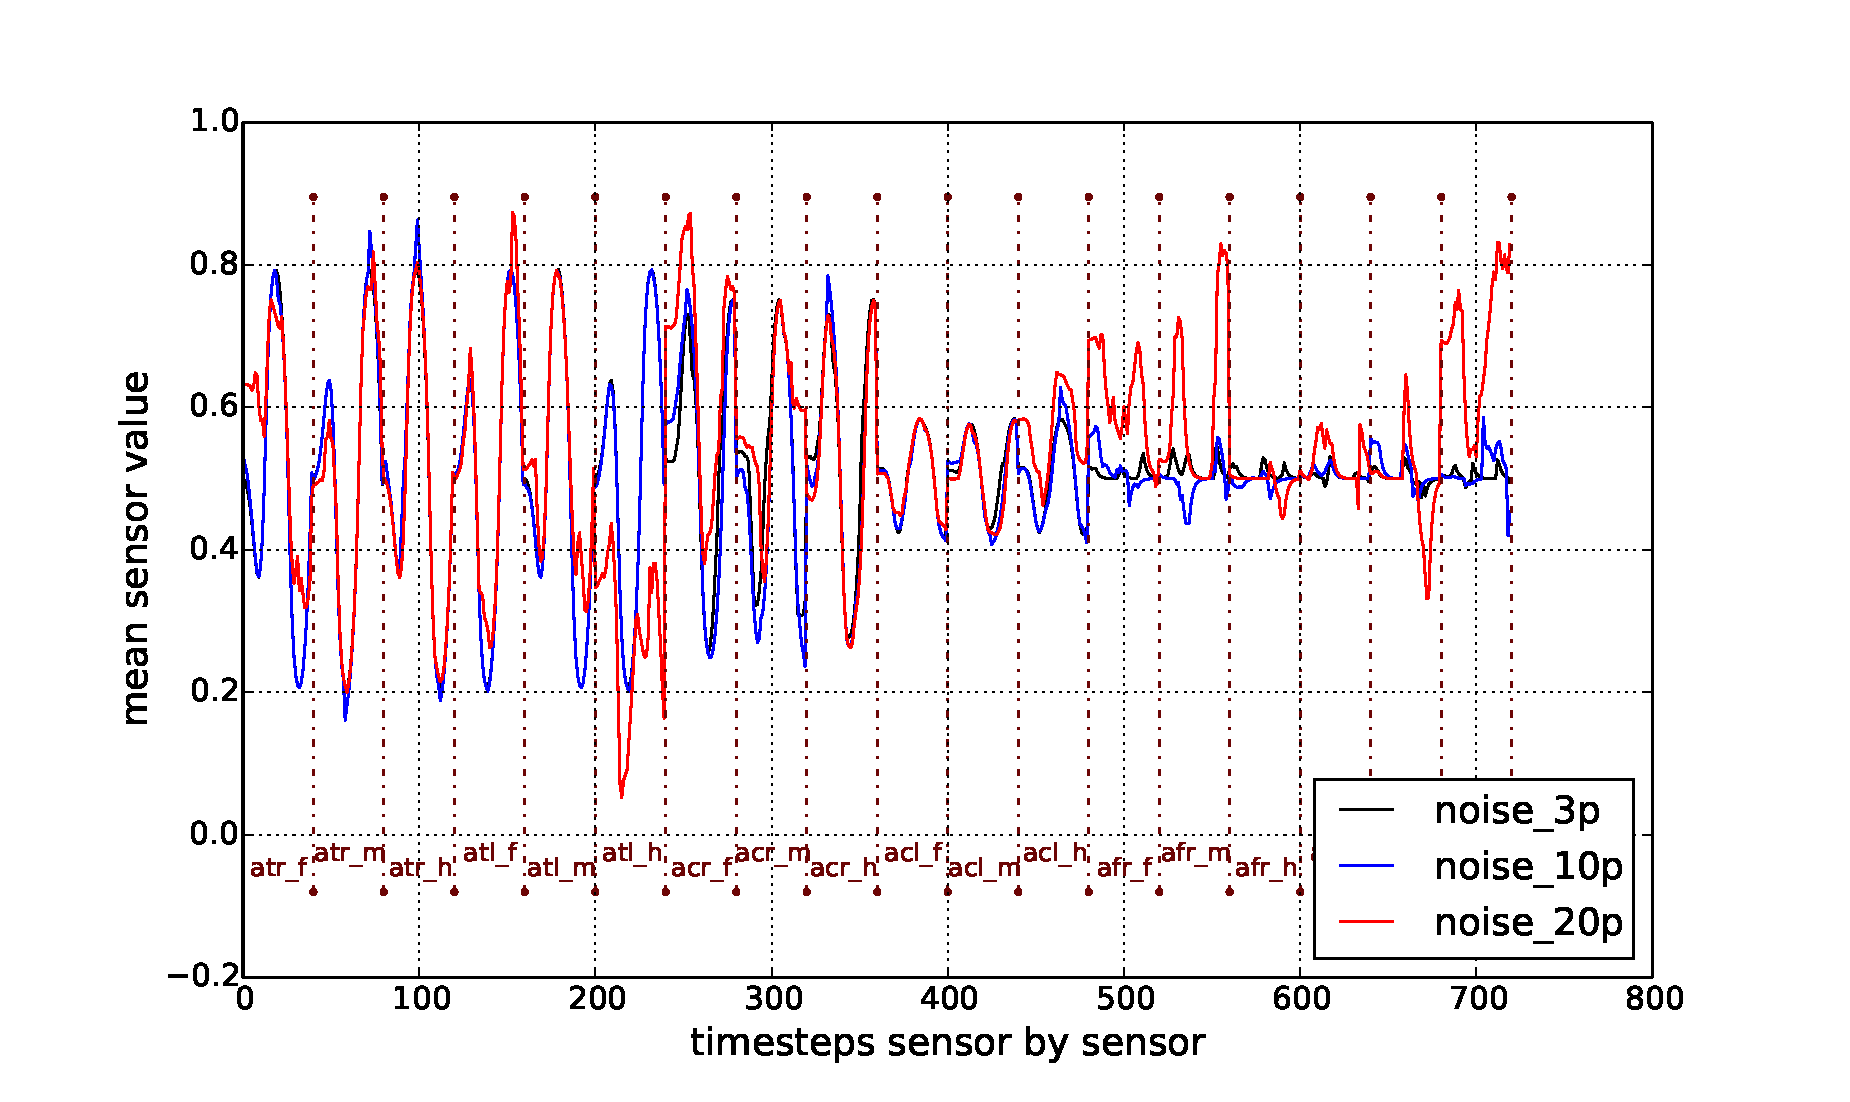
\includegraphics[width=1.0\textwidth]{tn_influence_samples_rock}
  \caption{Examples of noisy terrains: terrain rock, angle sensors}
  \label{fig:tn_influence_samples_rock}
\end{figure}

The purpose of adding the terrain noise is to generate a variability among samples of one terrain, which makes the terrain definition more flexible. As shown in \cref{fig:tn_influence_samples_rock}, the sample representing the $ 20\%-noise $ class fluctuates more in comparison to the others, expecially for the femur-tibia sensors. This might indicate a generation of an unusual rocky terrain.

\section{Data Acquisition} \label{sec:data_acquisition}
The data comes from the 18 proprioceptive and 6 tactile sensors and one needs to find a way how to form feature vectors (classification samples) out of it (\cref{sec:feature_vector_compilation}), which is one of the most essential parts of the process.

As it is later described in more detail, several sensors values in time need to be used to obtain the robot's dynamics on various terrains. Therefore, to generate a single data sample candidate, the simulation must be run for a period of time. We use the 'candidate' significaiton as the optimal duration of one sample is not known. Samples are then formed out of sample candidates.

To gather the data sample candidates, the simulator is launched several times in order to generate several candidates for every terrain type. It has been chosen to let the robot walk for $ 10 $ seconds each time, which leads to $ 100 $ values per sensor for one run (see simulation settings in \cref{ssec:app:lpzrobots_sim}).

As showin in \cref{img:amosii_leg}, the robot has $ 3 $ proprioceptive and $ 1 $ tactile sensor on each leg. In the following figures (\cref{fig:sensor_atr_f_no_noise} - \cref{fig:sensor_fr_f_no_noise}), examples for each of these sensor types are shown for all reffered terrains.

In \cref{fig:sensor_atr_f_no_noise}, outputs of the \textit{Thoraco-Coxal} joint angle sensor on the right front leg are shown. \textit{Thoraco} sensors produce similar outputs for all terrain types, however little variances (mostly for grass and carpet) can be seen.

\begin{figure}[H]
  \centering
  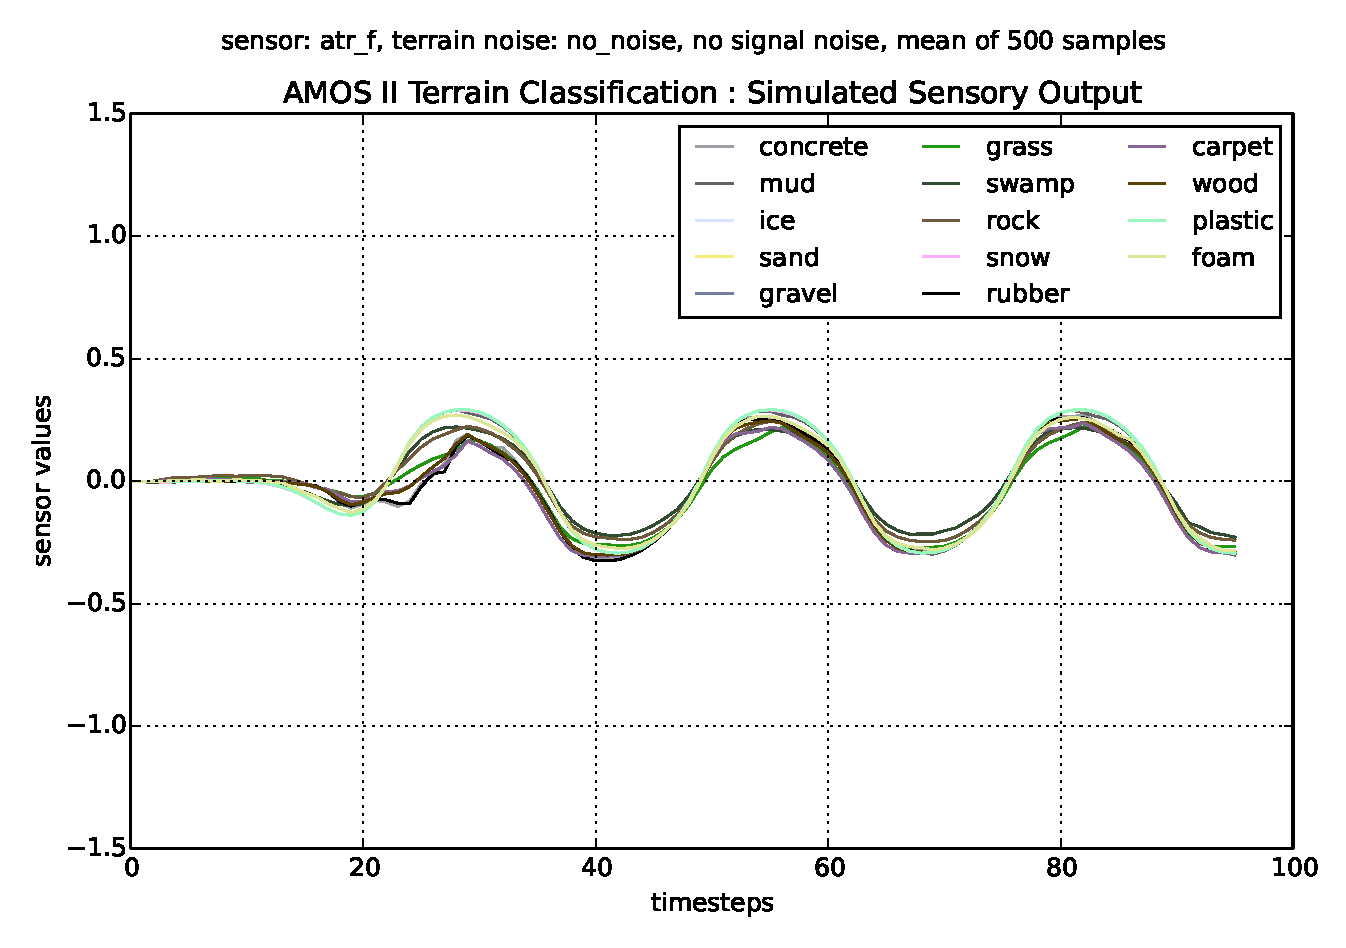
\includegraphics[width=1.0\textwidth]{sensor_atr_f_no_noise}
  \caption{Thoraco Sensor (ATRf) output examples, 14 terrains}
  \label{fig:sensor_atr_f_no_noise}
\end{figure}

\cref{fig:sensor_acr_m_no_noise} presents outputs of the \textit{Coxa-Trochanteral} joint angle sensor on the right middle leg. These joints are responsible for the elevation and depression of the leg and their signals vary especially at the decreasing parts of the signals. This might indicate that the leg is depressed differently on various terrains.

\begin{figure}[H]
  \centering
  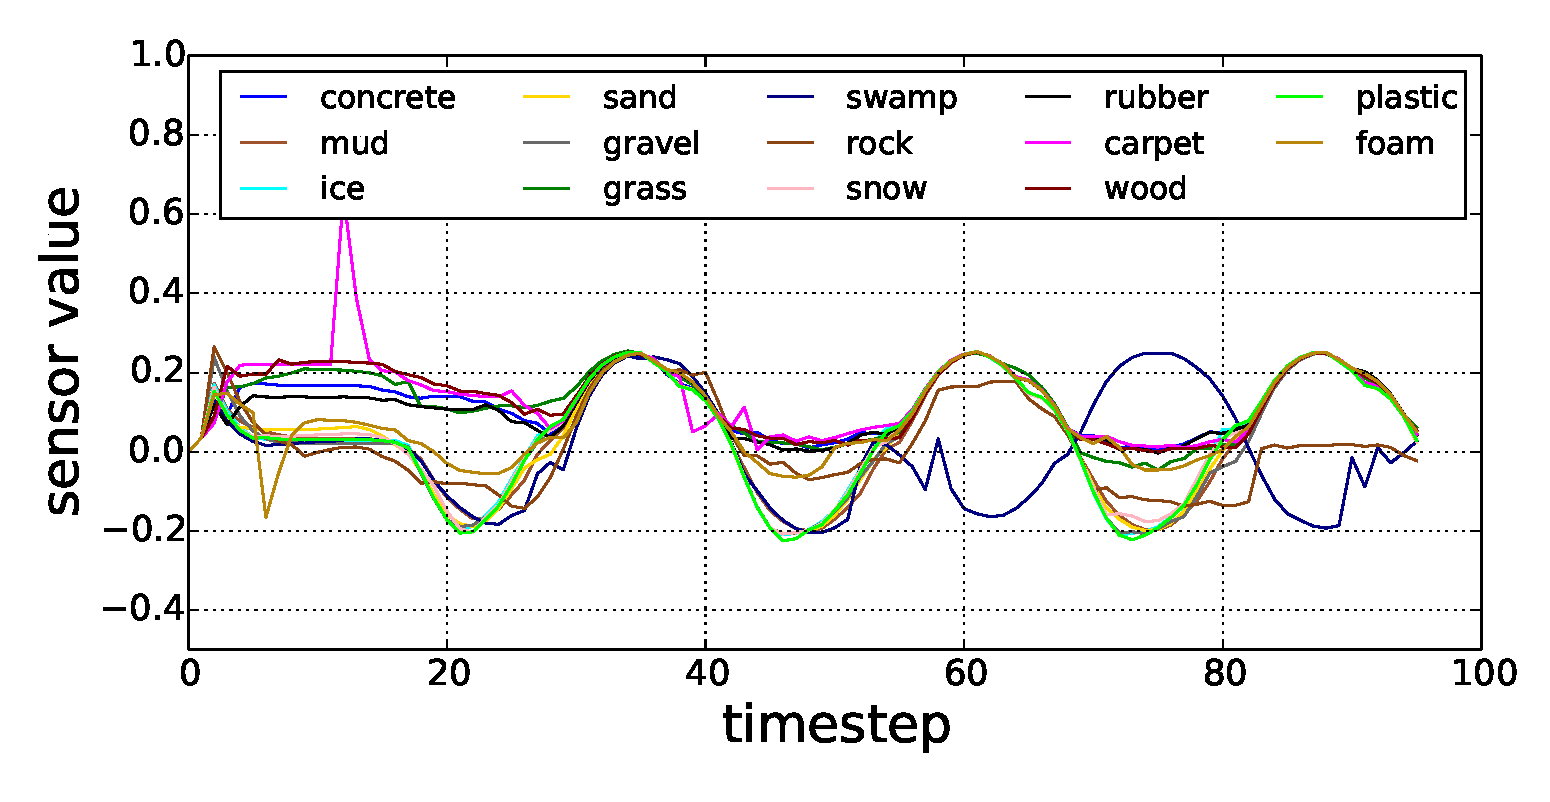
\includegraphics[width=1.0\textwidth]{sensor_acr_m_no_noise}
  \caption{Coxa Sensor (ACRm) output examples, 14 terrains}
  \label{fig:sensor_acr_m_no_noise}
\end{figure}

The \textit{Femur-Tibia} sensor outputs, for the joint sensor on the right hint leg, are illustrated in \ref{fig:sensor_afr_h_no_noise}. The signals indicate that this joint is not much used compared to previous ones. This makes sense as there is no active movement of this joint generated by the tripod gait controller (\cref{ssec:tripod_gait_controller}). The signals fluctuations must be caused by passive movements of the \textit{Femur-Tibia} joint, but still might be essential for classification.

\begin{figure}[H]
  \centering
  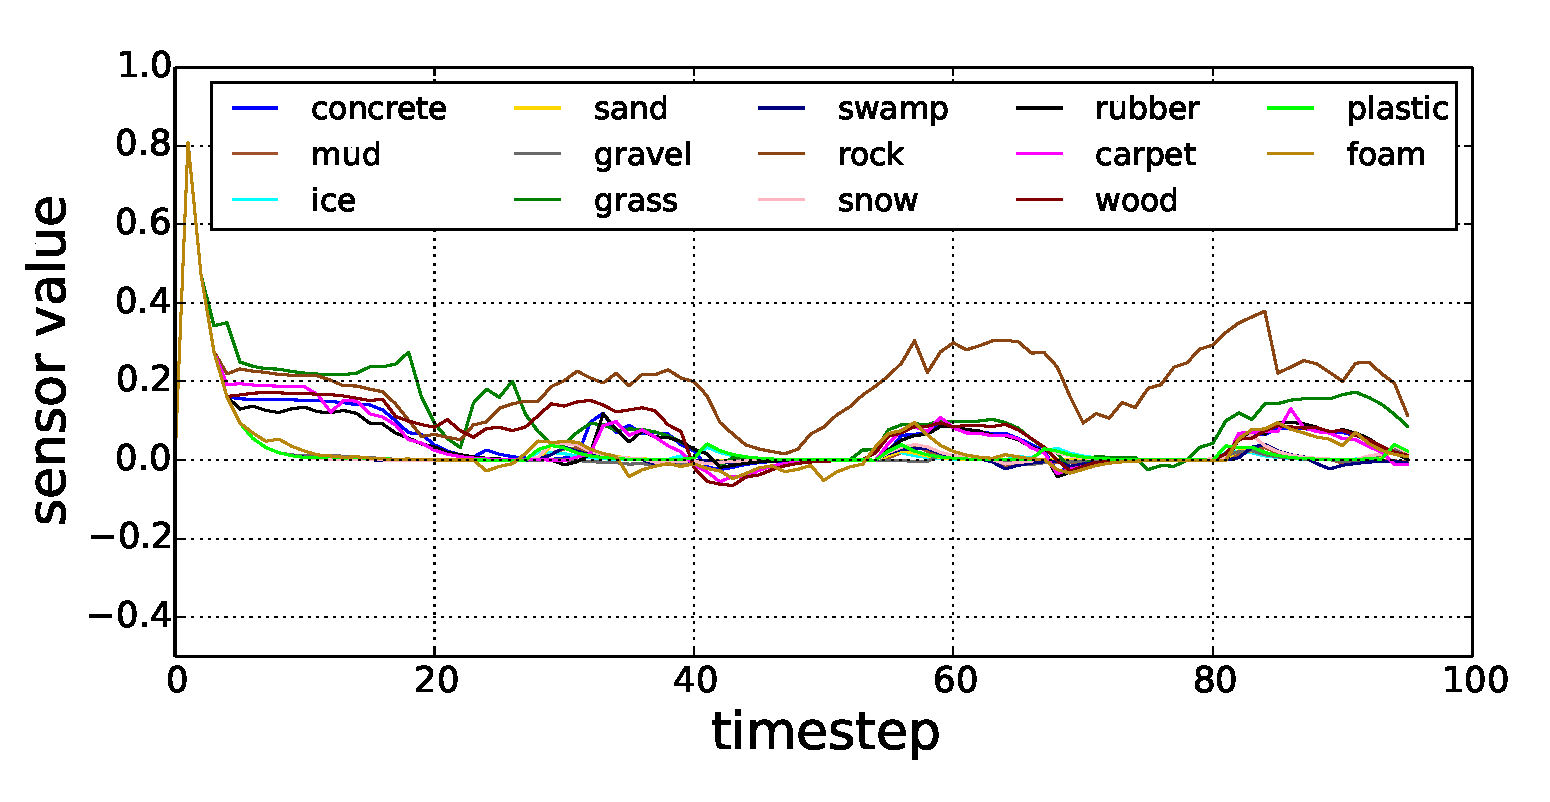
\includegraphics[width=1.0\textwidth]{sensor_afr_h_no_noise}
  \caption{Femur Sensor (AFRh) output examples, 14 terrains}
  \label{fig:sensor_afr_h_no_noise}
\end{figure}

The biggest variance among signals for various terrains is obtained from the foot contact sensors (example from the sensor on the right front leg in \cref{fig:sensor_fr_f_no_noise}). If the value of the foot contact sensor is $ 1 $, the robot stays on the foot with its full weight, and vice versa.

\begin{figure}[H]
  \centering
  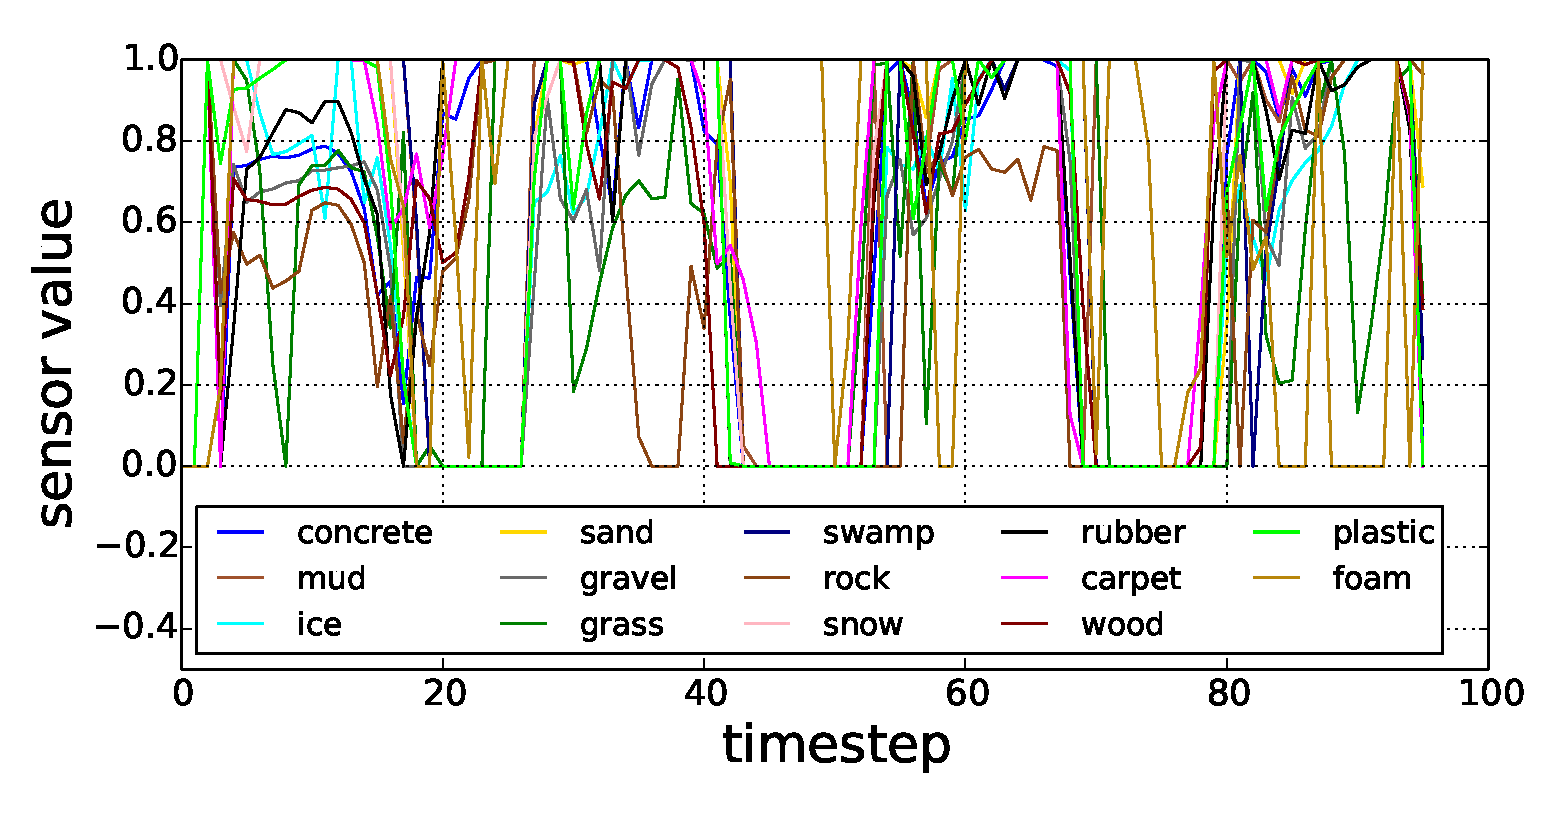
\includegraphics[width=1.0\textwidth]{sensor_fr_f_no_noise}
  \caption{Foot Contact Sensor (FRf) output examples, 14 terrains}
  \label{fig:sensor_fr_f_no_noise}
\end{figure}

Examples of signals from all 24 sensors can be found in \cref{sec:complete_sensory_data}.

As an optimal standard deviation value of the additive terrain noise is not known, some data for several values of this parameter have been generated. The simulation has been gradually run for:

\begin{itemize}
\item $ \sigma_p = 0.0 $ (no noise)
\item $ \sigma_p = 0.01 $ (1\% relative noise)
\item $ \sigma_p = 0.03 $ (3\% relative noise)
\item $ \sigma_p = 0.05 $ (5\% relative noise)
\item $ \sigma_p = 0.1 $ (10\% relative noise)
\item $ \sigma_p = 0.2 $ (20\% relative noise)
\end{itemize}

The $ \sigma_p $ corresponds to the $ std_p $ parameter used in \cref{eq:terrain_noise_generation}. The influence of additive terrain noise is analyzed in \cref{sssec:terrain_noise_influence}.

The approach of storing the gathered data is described in \cref{ssec:app:data_storing}. As \cref{img:data_dir_structure} shows, $ 500 $ sample candidates are generated for every \textit{noise/terrain} configuration. This allows creating datasets of $ 500 $ samples per class.

\section{Building a Feature Vector} \label{sec:feature_vector_compilation}
Classification tasks are generally based on datasets consisting of samples and corresponding targets. The samples need to be represented in a numerical way in order to be processed by a computer and its appropriate algorithms. In machine learning, this numerical representation of an object is called \textit{a feature vector}, an n-dimensional vector of numerical values. This section is devoted to building a feature vector out of the data gathered from proprioceptive and tactile sensors.

As the optimal structure is not known, several possibilities are tested and therefore some new global process parameters appear at this point (mentioned already in \cref{sec:overall_process_summary}).

For this particular problem, the task is to form one feature vector out of the content of one stored data file (see \cref{ssec:app:data_storing}), as each of these files contains data for one sample (see \cref{img:feature_vector_forming}).

\begin{figure}[H]
  \centering
  \includegraphics[width=1.0\textwidth]{feature_vector_forming}
  \caption{Forming a feature vector out of a data file.}
  \label{img:feature_vector_forming}
\end{figure}

It is assumed that a proper terrain classification using proprioceptors at one moment in time is at least difficult, if not impossible. Therefore the idea is to let the robot walk for a while and take down the dynamics of the sensors. Of course, the more timesteps are used for one sample, the more time the classification takes. Because of these arguments the number of timesteps is left as a global process parameter and it is a subject for later discussion.

Sensor selection defines another global process parameter. The anticipation is that the feature vector becomes redundant using all of the 24 sensors, as many of them may contain similar information. However, for now all of them are used to show how the feature vector is built and it is also left for later discussion.

With reference to \cref{img:feature_vector_forming}, feature vectors have been constructed by fixing the \textit{timesteps} parameter and concatenating columns of the matrix into one vector. This results into having data from all sensors one by one next to each other and forming one feature vector together. 

In \cref{fig:sample_example_normed} an illustration of the vector formation for three terrain types is shown. The number of timesteps is set to $ 40 $ and all $ 24 $ sensors are used, hence a feature vector of length $ 960 $ is obtained. The corresponding sensor abbreviations (see \cref{tab:proprioceptors}) are added to the x-axis annotation. The 18 angle sensors are followed by the 6 foot contact sensors.

\subsection{Feature Vector Normalisation} \label{ssec:normalisation}
It is a good manner to keep the data normalised - mapped to $ [0.0, 1.0] $ interval. The default range of foot contact sensors is already set to $ [0.0, 1.0] $, so there is nothing to change. For the joint angle sensors, the following approach, sometimes called \textit{feature scaling}, is used to map the data.

For each element $ S_i $ of signal $ S $:

\begin{align} \label{eq:normalisation}
S_i' = \frac{S_i - r_{min}}{r_{max} - r_{min}} 
\end{align}

\begin{description}
\item[$ r_{min}, r_{max} $] : bounds of the corresponding original sensor range (listed in \cref{tab:proprioceptors})
\item[$ S_i' $] : scaled element of the normalised signal
\end{description}

Also a $ [0, 1] $ interval overflow checking is added and values are adjusted if needed (\cref{eq:normalisation_overflow}). This is a cover for the case when ranges from \cref{tab:proprioceptors} were not accurate.

\begin{align} \label{eq:normalisation_overflow}
S_i' = min(max(S_i', 0), 1)
\end{align}

The following figure (\ref{fig:sample_example_normed}) shows normalised feature vector examples for three terrains. The influence of normalisation on classification results is another subject for the discussion.

\begin{figure}[H]
  \centering
  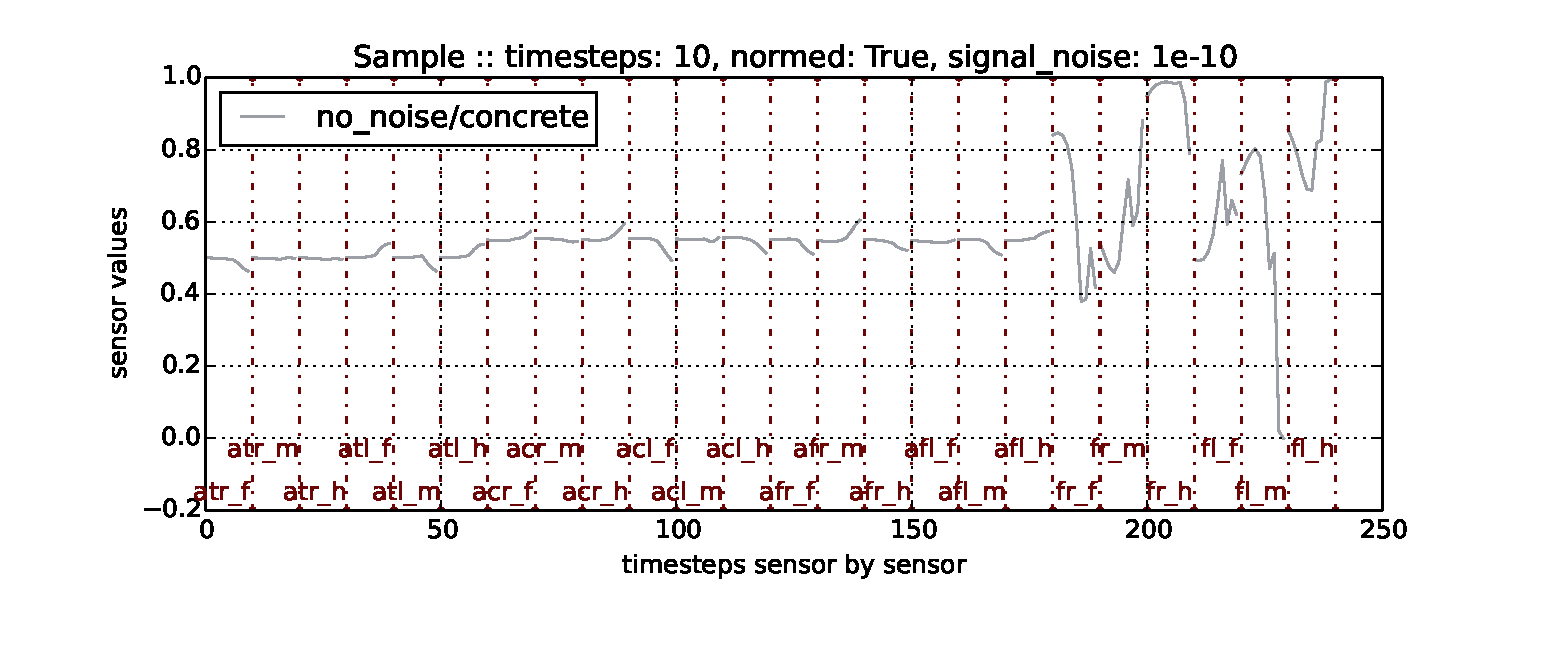
\includegraphics[width=1.0\textwidth]{sample_example_normed.eps}
  \caption{Normalised feature vector examples}
  \label{fig:sample_example_normed}
\end{figure}

\subsection{Signal Noise} \label{ssec:signal_noise}
In \cref{ssec:terrain_noise} a few general reasons for adding a noise to simulation data were disscused. In that case an additive Gaussian noise is used to generate variability in the data and to make the terrain types definitions (from \cref{tab:proprioceptors}) more general.

For similar reasons a signal noise is also added to the sensory data. In reality the data obtained from mechanical sensors are noisy (environmental conditions, failures of electrical devices, etc.), while the data coming from the simulated sensors are always deterministic.

In this case, a white Gaussian noise is added to the normalised feature vectors. Similarly to equations in \cref{ssec:terrain_noise}, at first a noise is generated using the normal distribution with zero mean and specified standard deviation. This time, a vector of length $ n $ needs to be generated as a noise.

\begin{align}
signal\_noise = [sn_1, sn_2, ..., sn_n]
\end{align}

\begin{align}
sn_i \sim N(\mu, \sigma^2), \quad i = 1, 2, ..., n
\end{align}

Then, the generated vector is added to a normalised feature vector from \cref{ssec:normalisation} (\cref{eq:signal_noise_addition}).

\begin{align} \label{eq:signal_noise_addition}
noised\_signal_i = raw\_signal_i + sn_i, \quad i = 1, 2, ..., n
\end{align}

Finally, the noised signal is checked, whether its values do not overflow out of the $ [0, 1] $ range.

\begin{align}
noised\_signal_i = min(max(noised\_signal_i , 0), 1), \quad i = 1, 2, ..., n
\end{align}

Also in this case, it is difficult to estimate an optimal signal noise power (standard deviation of the normal distribution). Therefore it is left as another global process parameter and its influence is discussed in the results part. It is defined as a percentage of the $ [0.0, 1.0] $ interval and as the signals are normed in advance, there is no need for another processing of this parameter.

\subsubsection*{Influence of Signal Noise} \label{sssec:signal_noise_influence}
\cref{fig:sn_influence_samples_concrete} shows the influence of the signal noise on one sample of \textit{concrete} for joint angle sensors. A similar figure for foot contact sensors is put in \cref{sec:further_data_analysis} (\cref{fig:sn_influence_samples_concrete_fc}).

Naturally, the higher the standard deviation of additive Gaussian noise is, the more a corresponding signal fluctuates around the \textit{red signal} representing no signal noise.

\begin{figure}[H]
  \centering
  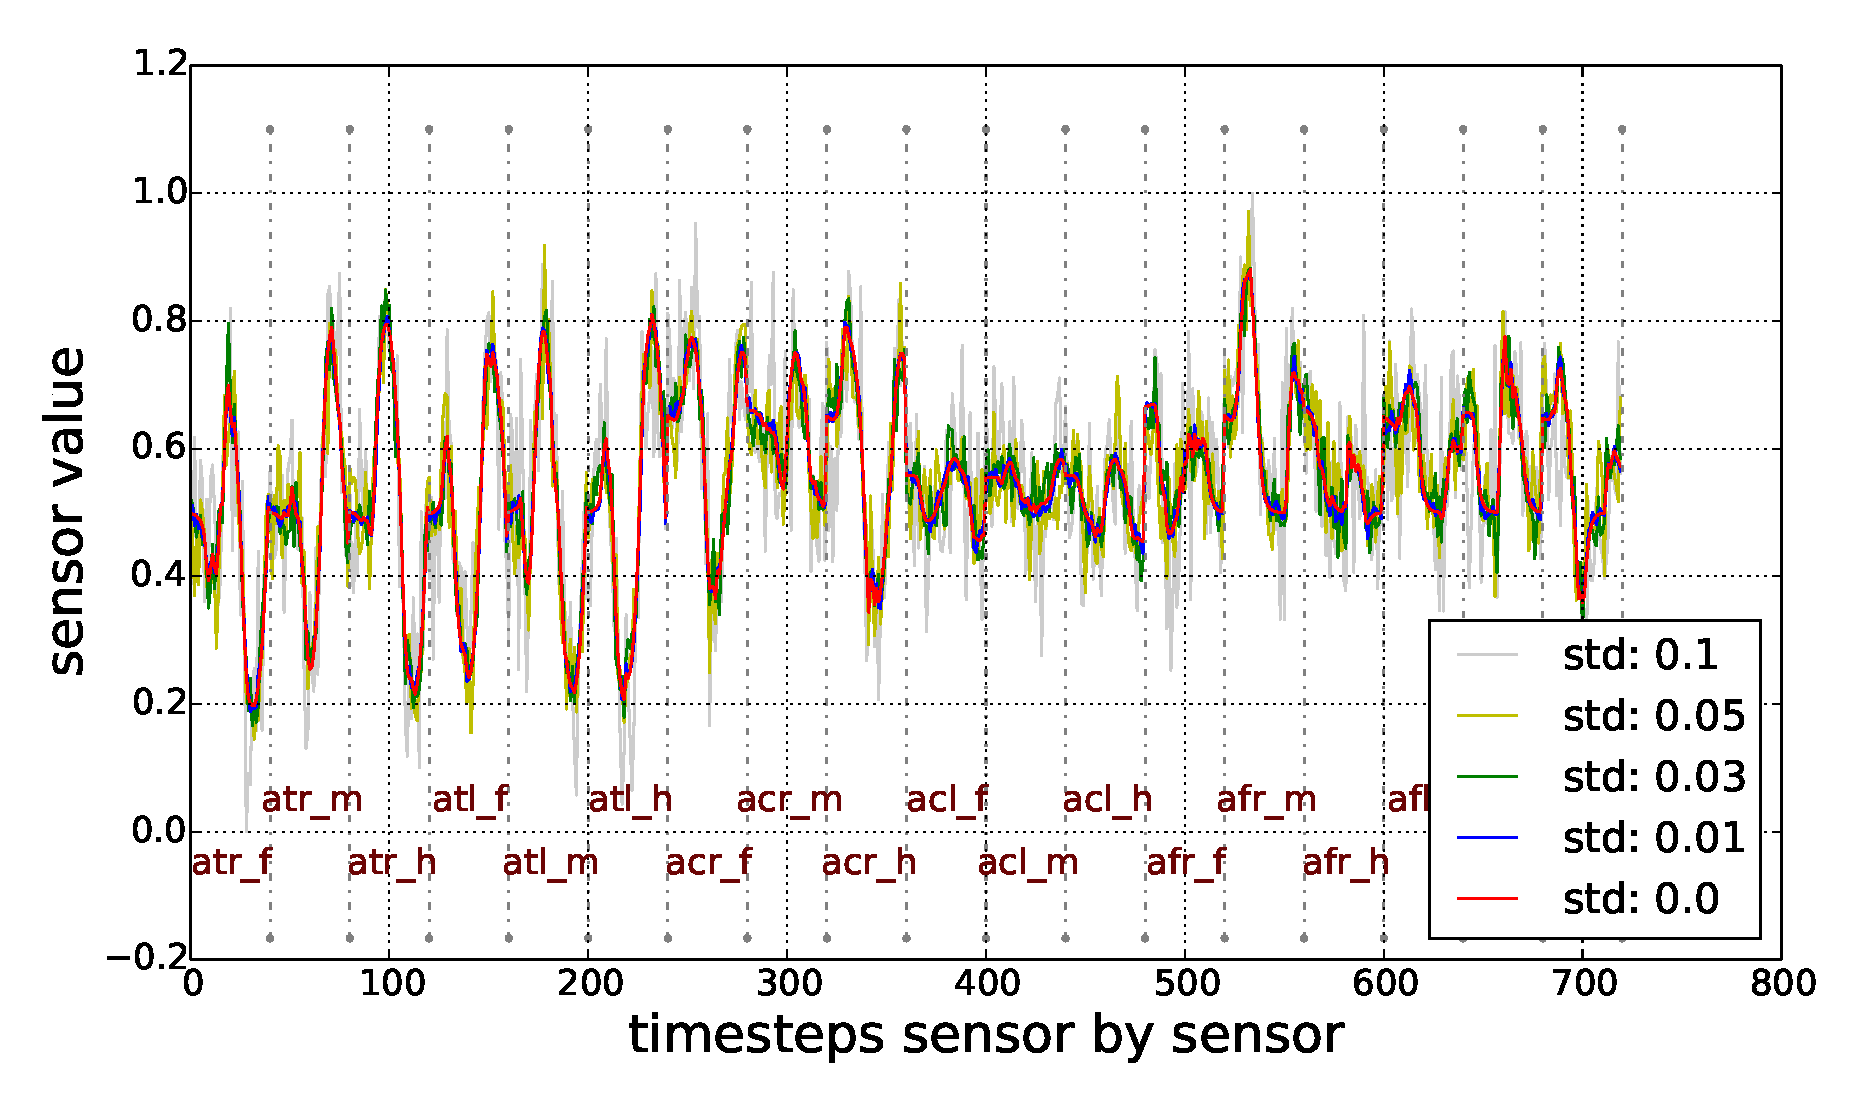
\includegraphics[width=1.0\textwidth]{sn_influence_samples_concrete}
  \caption{Examples of noisy signals: concrete, angle sensors}
  \label{fig:sn_influence_samples_concrete}
\end{figure}

\section{Generation of Datasets} \label{sec:dataset_creation}
In this section, the task is to transform all the data into so called datasets. There are usually three sets of data used for classification tasks - training, validation and testing data. These three sets must be disjunctive, meaning they cannot have a single element in common. All these three sets together form a dataset.

\begin{figure}[H]
  \centering
  \includegraphics[width=0.8\textwidth]{three_sets}
  \caption{Three sets of data in a dataset.}
  \label{img:three_sets}
\end{figure}

Each set of data consists of samples and targets (class labels). The samples are represented by normalised feature vectors (\cref{sec:feature_vector_compilation}) - lists of numerical floating point values from $ [0.0, 1.0] $ interval. Every sample must be uniformly assigned to precisely one target. The targets, in this case, match the virtually created terrain types (listed in \cref{tab:terrains_parameters}) in the following manner.

The target vector is of length 14, as there are 14 terrain types. Every terrain type has an unique identificator (numbers listed in \cref{tab:proprioceptors}) corresponding to positions in the target vector. In any case, the vector contains 13 'zeros' and 1 'one'. The vector is then matched to a terrain type depending on the position where the 'one' is. For instance, a target vector corresponding to \textit{concrete} is illustrated on \cref{img:target_vector_concrete}.

\begin{figure}[H]
  \centering
  \includegraphics[width=0.4\textwidth]{target_vector_concrete}
  \caption{Target vector for concrete}
  \label{img:target_vector_concrete}
\end{figure}

Once there are two ordered lists - a list of samples and a corresponding list of targets, these lists are split into the three sets shown in \cref{img:three_sets}. There is a parameter called \textit{data\_split\_ratio} defining the proportions among the sets sizes. By default the ratio is set to generate 80\% training, 10\% validation and 10\% of testing data.

\begin{figure}[H]
  \centering
  \includegraphics[width=0.8\textwidth]{create_dataset}
  \caption{Workflow of generating a dataset}
  \label{img:create_dataset}
\end{figure}

The workflow of data generation procedure is illustrated in \cref{img:create_dataset}. 

\section{Training and Classification}
Having a dataset enables to train a classifier, a machine learning tool that is able to learn some behavior on one part of some data (training and validation) and then perform similarly on another "never seen" part of the data (testing) - as shown in \cref{img:three_sets}.

There are many classification methods differing in mathematical backgrounds and each of them has some adventages and disadvantages on various types of data. However, all of them have some general functionalities that comply with some kind of convention. For instance, there are at least two procedures that every classifier should be capable of:

\begin{description}
\item[model fitting] : In this procedure, an initialized classifier is usually given training samples and their corresponding targets. Additiionally, it can take some validation data and/or learning parameters. Then a model is trained using some math behind the selected classification method.
\item[unlabeled observation prediction] : Once the model is trained, it is capable of predicting classes of unlabeled samples. It takes one or more samples of testing data and returns the predicted target(s).
\end{description}

This convention enables testing different classification approaches on the same data in the same way. Therefore also the implemented network library \textit{kitt\_nn} (see \cref{chap:kitt_nn}) provides these functions and is capable of working with datasets of the same structure as the public \textit{.py} classifiers (discussed in sections \ref{ssec:sknn} and \ref{ssec:other_classifiers}).

In the overall process diagram (\cref{img:terrain_overall_simple}) there is a box called \textit{classification with full networks}. The procedure behind this box is illustrated on \cref{img:train_and_test_network}.

\begin{figure}[H]
  \centering
  \includegraphics[width=0.8\textwidth]{train_and_test_network}
  \caption{Procedure of training and testing a network}
  \label{img:train_and_test_network}
\end{figure}

This workflow is performed by the implemented framework \textit{kitt\_nn} (\cref{chap:kitt_nn}, as well as by other provided classifiers (discussed in \cref{ssec:other_classifiers}) for comparison. It is adventageous, that each of these tools can use the same workflow and so the comparison is fair.

There are several arguments (firstly listed in \cref{sec:overall_process_summary}) that differentiate the final trained networks and their performances. The first one is the dataset that the network is trained on. This parameter brings its own configuration (see its input parameters in \cref{img:create_dataset}) and so its setting parametrizes the classifier as well.

Next, one needs to define the network initial structure in sense of number of hidden layers and number of neurons in each of these layers. The input and output layers are determined by the dataset. There are many parameters to be defined for learning like \textit{batch size}, \textit{initial random state} etc. In this work, only the learning rate and the number of epochs are used as training parameters. The learning process follows the implemented backpropagation algorithm described in \cref{sec:learning_algorithm}.

\subsection{Other Classification Methods for Comparison} \label{ssec:other_classifiers}
\textbf{TODO :} describe here how other classifiers have been tested and reffer to the results part

SVM, k-NN, RandomForest

\subsection{Evaluation Measures} \label{ssec:evaluation_measures}
A trained network is evaluated on testing data. This evaluation provides a set of the most important classification metrics \citep{article:scikit-learn}.

\begin{description}
\item[accuracy] : the set of labels predicted for a sample must exactly match the corresponding set of true labels
\item[precision] : ability of the classifier not to label as positive a sample that is negative
\item[recall] : the ability of the classifier to find all the positive samples
\item[F1 score] is interpreted as a weighted average of the precision and recall, where an F1 score reaches its best value at 1 and worst score at 0. The relative contribution of precision and recall to the F1 score are equal. Formula:
\begin{equation} \label{eq:f1_score}
F1 = \frac{2 * precision * recall}{precision + recall}
\end{equation}
\item[confusion matrix] : a confusion matrix $ C $ is such that $ C_{i, j} $ is equal to the number of observations known to be in group $ i $ but predicted to be in group $ j $.
\item[classification error] : DESCRIBE (formula).
\item[average epoch time] : DESCRIBE.
\item[evarage classification time] : DESCRIBE.
\end{description}

structure, n synapses ?